\section{Matrix Factorization}  \label{sec:mf}

% need update and to be consistent with related work 
Given a data matrix of observed and missing entries, the essence of Matrix Factorization~(MF) is to learn latent factors from the observed entries, and then leverage these factors to predict the missing entries.
MF is one of the most successful Collaborative Filtering~(CF) models in the area of Recommendation Systems.
In CF, where we consider the rows of the matrix as users and the columns as items, and we wish to predict unknown item ratings by users which reflect known user preferences.
The unknown rating prediction in CF is much like missing data recovery in Wireless Sensor Networks~(WSN), except the rows become time steps, the columns become sensor nodes, and the data characteristic is different. 

In the following discussion, we will introduce the fundamentals of the MF methodology, communicate our novel sensor network data specific modifications to the MF objective function, and finally provide the complete procedure of our proposed method.

\subsection{Basic Formulation of Matrix Factorization}

The approach of MF is strongly related to Singular Value Decomposition~(SVD).
SVD decomposes a completely observed matrix~$\mathbf{R}$ into one diagonal matrix~$\mathbf{D}$ and two unitary matrices~$\mathbf{U}$ and~$\mathbf{V}$ such that
\begin{equation*} \mathbf{R} = \mathbf{U}\mathbf{D}\mathbf{V}^T. \end{equation*}
The largest $K$ singular values, $\mathbf{U}_K \mathbf{D}_K \mathbf{V}_K^T$, form the best $K$-rank approximation of $\mathbf{R}$ under the Frobenius Norm. 

Conventional SVD is undefined when the matrix~$\mathbf{R}$ is incomplete.
Recent research shows\cite{koren2009matrix} that when the matrix~$\mathbf{R}$ is partially observed, a better approach is to factorize $\mathbf{R}$ by considering observed entries only.
Utilizing numerical optimization procedures, we generate two small matrices~$\mathbf{P}_{MK}$ and $\mathbf{Q}_{KN}$ that approximate the observed entries of $\mathbf{R}_{MN}$
\begin{equation*}\mathbf{R} \approx \mathbf{P} \mathbf{Q}.\end{equation*}
If $\mathbf{R}$ is a matrix of temperature readings, then each row of $\mathbf{P}$ represents latent factors of the time step and each column of $\mathbf{Q}$ is the latent factors of the sensor node.

We adopt the biased-MF which includes row and column biases $\mu_m$ and $\mu_n$. % is added for predicting $r_{m,n}$.
In a temperature monitoring system, the row bias can be understood as the average temperature at a given time, and the column bias reflects the systematic bias of the sensor node.
Therefore, we have the prediction $\hat{r}_{m,n} = \mu_m + \mu_n + \mathbf{p}_m \mathbf{q}_n$.
After adding the regularization term, the whole objective function becomes
\begin{equation*}\begin{aligned}
\frac{1}{2}\sum_{m,n}{(r_{m,n} - \hat{r}_{m,n})}^2 & + \frac{\beta_1}{2}\sum_m{\mu_m^2} + \frac{\beta_2}{2}\sum_n{\mu_n^2}\\
& + \frac{\beta_3}{2}\sum_m{||\mathbf{p}_m||^2} + \frac{\beta_4}{2}\sum_n{||\mathbf{q}_n||^2}.\\
\end{aligned}\end{equation*}
In the equation, $\mathbf{p}_m$ are the row factors of $\mathbf{P}$ (for time $m$), and $\mathbf{q}_n$ are the column factors of $\mathbf{Q}$ (for sensor node $n$) respectively.
$\beta_1$, $\beta_2$, $\beta_3$, $\beta_4$ are parameters that control the strength of regularization.

\subsection{Temporally-Regularized Matrix Factorization}

\begin{figure}[htbp]
	\centering
	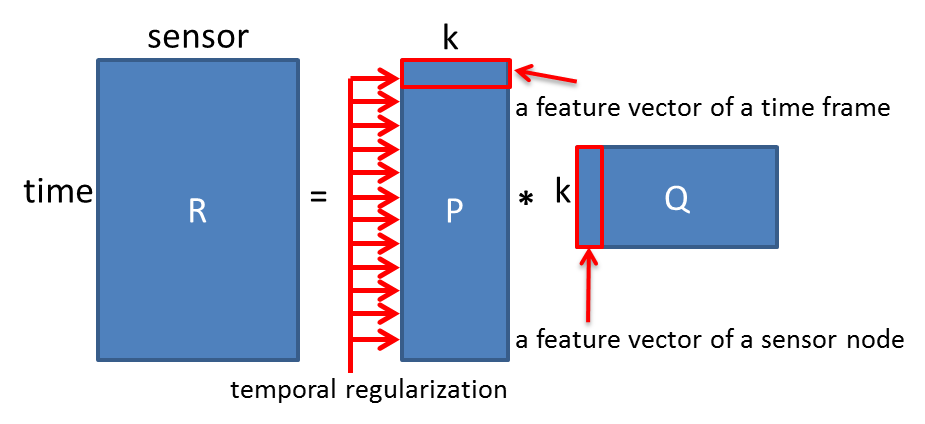
\includegraphics[width=0.5\textwidth]{TRMF_illustration.png}
	\caption{illustration of TR-MF}
\end{figure}

%cite temporal reference

Although the goals of both CF and WSN data recovery are unobserved entry prediction, the data characteristics are very different.
In typical recommender systems, users and items may each be on the order of millions.
In contrast, for missing WSN data estimation, there are usually a large number of time steps, with much smaller number of sensor nodes.
The inter-sensor correlations may be easily learned from the data by the CF technique, but the temporal correlation is not considered.
In particular, users and items are independent in CF, while WSN time steps have a fixed order, where nearer time steps have a stronger correlation.
With this observation, we define Temporally-Regularized Matrix Factorization (TR-MF) to better fit the characteristic of WSN data. 

As the name may suggest, TR-MF adds a temporal regularization term to conventional MF.
The temporal regularization forces the bias terms and features of adjacent rows to be similar, which reflects our intuition that readings in adjacent time steps should be similar.
To achieve this effect, we modify our objective function as follows 
\begin{equation*}\begin{aligned}
\frac{1}{2}\sum_{m,n}{(r_{m,n} - \hat{r}_{m,n})}^2 &+ \frac{\beta_1}{2}\sum_m{\mu_m^2} + \frac{\beta_2}{2}\sum_n{\mu_n^2}\\
&+ \frac{\beta_3}{2}\sum_m{||\mathbf{p}_m||^2} + \frac{\beta_4}{2}\sum_n{||\mathbf{q}_n||^2}\\ 
&+ \frac{1}{2}\gamma_1\sum{(\mu_m-\mu_{m+1})^2} + \frac{1}{2}\gamma_2\sum{||\mathbf{p}_m-\mathbf{p}_{m+1}||^2}.
\end{aligned}\end{equation*}

\subsection{Optimization Procedure of TR-MF}
\label{optimation_procedure}
Several MF solving methodologies have been proposed, such as Stochastic Gradient Descent (SGD)\cite{koren2009matrix,chih2008large}, Alternating Least Square (ALS)\cite{koren2009matrix,zhou2008large} and Newton's method\cite{buchanan2005damped}.
In our work, we utilize SGD for its efficiency and simplicity. 

In SGD, we incrementally update our model by considering one observed entry at a time.
Focused on one observed reading $r_{m,n}$, the objective function of MF is
\begin{equation*} \frac{1}{2}(r_{m,n} - \hat{r}_{m,n})^2 + \frac{\beta_1}{2}\mu_m^2 + \frac{\beta_2}{2}\mu_n^2 + \frac{\beta_3}{2}||\mathbf{p}_m||^2 + \frac{\beta_4}{2}||\mathbf{q}_n||^2\end{equation*}
Thus, the update equation is\\
$\begin{cases}
	\mu_m' = \mu_m - \eta_1 ((\hat{r}_{m,n}-r_{m,n}) + \beta_1 \mu_m) \\
	\mu_n' = \mu_n - \eta_1 ((\hat{r}_{m,n}-r_{m,n}) + \beta_2 \mu_n) \\
	\mathbf{p}_{m}' = \mathbf{p}_{m} - \eta_2 ((\hat{r}_{m,n}-r_{m,n})\mathbf{q}_{n} + \beta_3 \mathbf{p}_{m})\\
	\mathbf{q}_{n}' = \mathbf{q}_{n} - \eta_2 ((\hat{r}_{m,n}-r_{m,n})\mathbf{p}_{m} + \beta_4 \mathbf{q}_{n})\\
\end{cases}$\\
After we use every rating in the training set once, we update the model according to the temporal regularization
$\begin{cases}
	\mu_u' = \mu_u - \eta_1 \gamma_1((\mu_u-\mu_{u-1})+(\mu_u-\mu_{u+1}))\\
	\mathbf{p}_{u}' = \mathbf{p}_{u} - \eta_2 \gamma_1((\mathbf{p}_{u}-\mathbf{p}_{u-1})+(\mathbf{p}_{u}-\mathbf{p}_{u+1}))\\
\end{cases}$

We summarize our algorithm in \textbf{Procedure \ref{alg:TRMF}} and provide details in the following sections.

\paragraph*{Data Normalization}

Unlike the rating scores in CF which have a fixed range, readings from WSN are real-valued, and the range may vary with situation.
Before training, we normalize the training set by its mean and variance, and in training we update the model by the normalized training set.
While predicting the validation set and testing sets, we restore the prediction to the original mean and variance range and then calculate the error.

There are two benefits to performing data normalization.
When the global mean becomes zero, the origin of our model becomes a good initial point.
This initial point impacts the performance of MF greatly because the MF objective function finds only a local minimum (i.e.\ the formulation is non-convex).
Secondly, normalization forces different data sets to look similar which simplifies the parameter tuning task for TR-MF and is the foundation of Multivariate TR-MF (Section \ref{subsec:Multivariate_TRMF}). 


\paragraph*{Initialization}

There are three ways to initialize the bias terms:
\begin{enumerate}
	\setlength {\itemsep}{-5pt}
	\item Set all of them to zeros.
	\item Set the row bias as the row mean, and then set the column bias as the column mean of every reading minus its row bias.
	\item Opposite procedure as previous.
\end{enumerate}
For all components of every $\mathbf{p}_{u}$ and $\mathbf{q}_{i}$, we set them to ~$\mbox{random}(-0.05,0.05)/K$, where $K$ is number of features.

\paragraph*{Parameters}

We seem to have many parameters: conventional regularization for user bias~$\beta_1$, item bias~$\beta_2$, user feature~$\beta_3$, item feature~$\beta_4$, temporal regularization term for bias~$\gamma_1$ and for feature~$\gamma_2$, learning rate for bias~$\eta_1$ and for feature~$\eta_2$, number of features~$K$, but in many cases we can achieve reasonable performance by setting 
\begin{equation*}\beta_1 = \beta_2 = \beta_3 = \beta_4, \gamma_1 = \gamma_2, \eta_1 = \eta_2. \end{equation*}
Which we use as the setting in our experiment.
We share our experience about setting parameters in \textbf{Section \ref{subsec:parameter}}.

\paragraph*{Stopping Criterion}

To decide when to cease updating the MF model, we use the validation set and cease training when the validation error is increasing and the current iteration number minus the best iteration number is greater than a threshold (we use an iteration threshold of $500$). 

\begin{algorithm}
	\caption{Temporally-Regularized Matrix Factorization}
	\label{alg:TRMF}
	\textbf{Parameter:} $\beta_1$, $\beta_2$, $\beta_3$, $\beta_4$, $\gamma_1$, $\gamma_2$, $\eta_1$, $\eta_2$, $K$\\
	\textbf{Input:} training set, validation set
	\begin{algorithmic}
		\State Normalize the training set as $\mathcal{D}$
		\State Initialize $\mu_m$, $\mu_n$, $\mathbf{p}_m$, $\mathbf{q}_n$ for all $m$, $n$
		\Repeat
			\State \textbf{for} each observed reading $r_{m,n}$ in $\mathcal{D}$
				\State \indent Update $\mu_m$, $\mu_n$, $\mathbf{p}_{m}$, $\mathbf{q}_{n}$
			\State Update $\mu_m$, $\mathbf{p}_m$ for every $m$ by temporal regularization
		\Until{stopping criterion is met}
		\State Output the model for testing set prediction
	\end{algorithmic}
\end{algorithm}
